%%%%%%%%%%%%%%%%%%%%% chapter.tex %%%%%%%%%%%%%%%%%%%%%%%%%%%%%%%%%
%
% sample chapter
%
% Use this file as a template for your own input.
%
%%%%%%%%%%%%%%%%%%%%%%%% Springer-Verlag %%%%%%%%%%%%%%%%%%%%%%%%%%


\chapstarthook{El contenido del cap�tulo corresponde con el art�culo: \textbf{J.A. Aguilar, I. Garrig{\'o}s, J.-N. Maz{\'o}n. Impact Analysis of Goal-Oriented Requirements in Web Engineering. The 11th  International Conference on Computational Science and Its Applications (ICCSA 2011), June 20-23, 2011, Santander, Spain. Part V, Lecture Notes in Computer Science, Vol. 6786, pp. 421-436, 2011.}}


\chapter{Impact Analysis of Goal-Oriented Requirements in Web Engineering}
\label{c5} % Always give a unique label
% use \chaptermark{}
% to alter or adjust the chapter heading in the running head

%The previous chapters begin by defining multidimensional models at
%the conceptual level. However successful data warehouse design needs
%to be based upon a requirement analysis phase if it is to adequately
%represent the information needs of decision makers. Moreover, since
%the data warehouse integrates the information provided by data
%sources, it is also crucial to take these sources into account
%throughout the development process in order to obtain a consistent
%reconciliation of data sources and information needs. In this
%chapter, a requirement analysis approach for multidimensional
%modeling of data warehouses and the corresponding reconciliation
%process is developed. The content of this chapter corresponds with
%the part of the approach shaded in the figure below.


\begin{figure}[h!]
  \begin{center}
    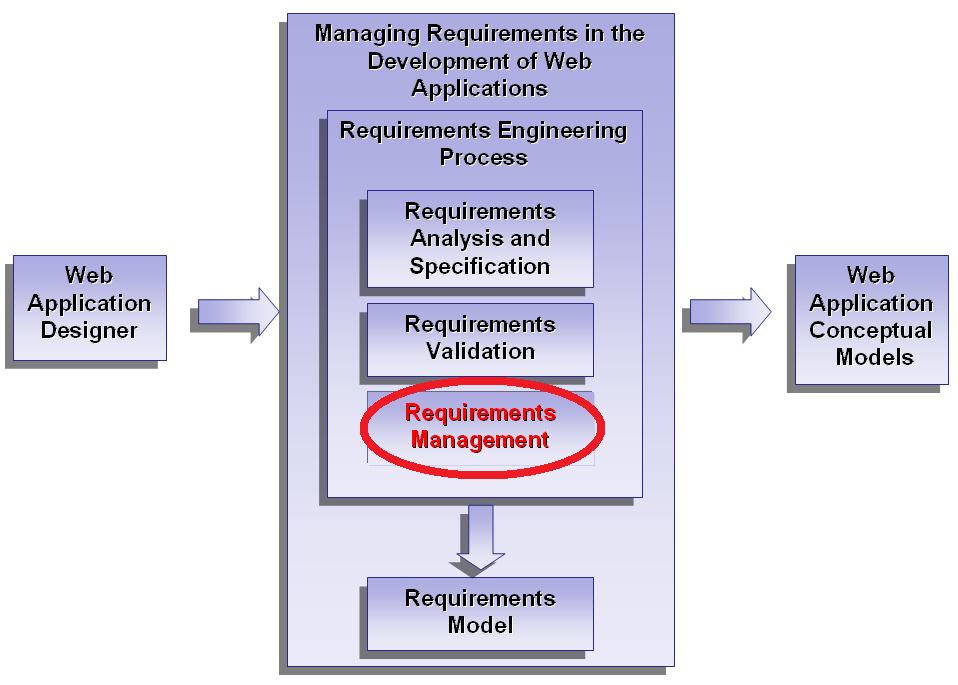
\includegraphics[width=0.7\textwidth]{img/PropuestaCap3.png}
  \end{center}
  %\caption{} \label{}
\end{figure}

%En el Cap�tulo \ref{c4} se present� una propuesta para el an�lisis y especificaci�n de requisitos en ingenier�a Web. 

En cap�tulos anteriores se ha resaltado la importancia de la etapa de an�lisis y especificaci�n de requisitos en la ingenier�a Web, obligada, principalmente, por las caracter�sticas particulares de este tipo de aplicaciones, tales como su audiencia heterog�nea y por la evoluci�n constante en las tecnolog�as de implementaci�n. Este tipo de caracter�sticas originan que la aplicaci�n Web sea propensa a sufrir cambios, por eso, es importante conocer en qu� medida impactar�n los cambios a los requisitos, as� como qu� partes de la aplicaci�n Web se ver�n afectadas. Para lograrlo, es necesario comprender y analizar las dependencias entre los requisitos, es decir, cuales requisitos est�n relacionados o cuales dependen uno del otro para cumplirse y con ello brindar soporte al dise�ador por medio de una mejor gesti�n y mantenimiento de la aplicaci�n Web. 

En este cap�tulo, se presenta un algoritmo para manejar las dependencias entre los requisitos funcionales y los requisitos no-funcionales de la aplicaci�n Web en un contexto orientado a objetivos (\emph{goal-oriented}). Con el algoritmo, es posible comprender cu�l es el impacto en los requisitos procedente de un cambio en la estructura de modelos conceptuales que conforman la aplicaci�n Web, as� como saber qu� requisitos necesitan ser implementados para cumplir, en medida de lo posible, los prop�sitos establecidos en el an�lisis orientado a objetivos.

%The content of this chapter corresponds with a paper published in
%the \emph{Data \& Knowledge Engineering (DKE)} journal. This reaches
%a world-wide audience of researchers, designers, managers and users.
%The major aim of the journal is to identify, investigate and analyze
%the underlying principles in the design and effective use of
%database and knowledgebase systems. This journal publishes original
%research results, technical advances and news items concerning data
%engineering, knowledge engineering, and the interface of these two
%fields. It should also be mentioned that this journal had an
%\emph{impact factor} of \emph{1.144} in 2007, according to the
%\emph{Thomson's Science Citation Index (SCI)}
%(\url{http://www.isiwebofknowledge.com/}).

%Finally, it is worth mentioning that this paper has been ranked by
%\emph{ScienceDirect} (\url{http://www.sciencedirect.com/}) as one of
%the \emph{25 hottest articles} published in DKE during last quarter
%of 2007 (\url{http://top25.sciencedirect.com}).
%(\url{http://top25.sciencedirect.com/subject/engineering/12/journal/data-knowledge-engineering/0169023X/archive/14/})


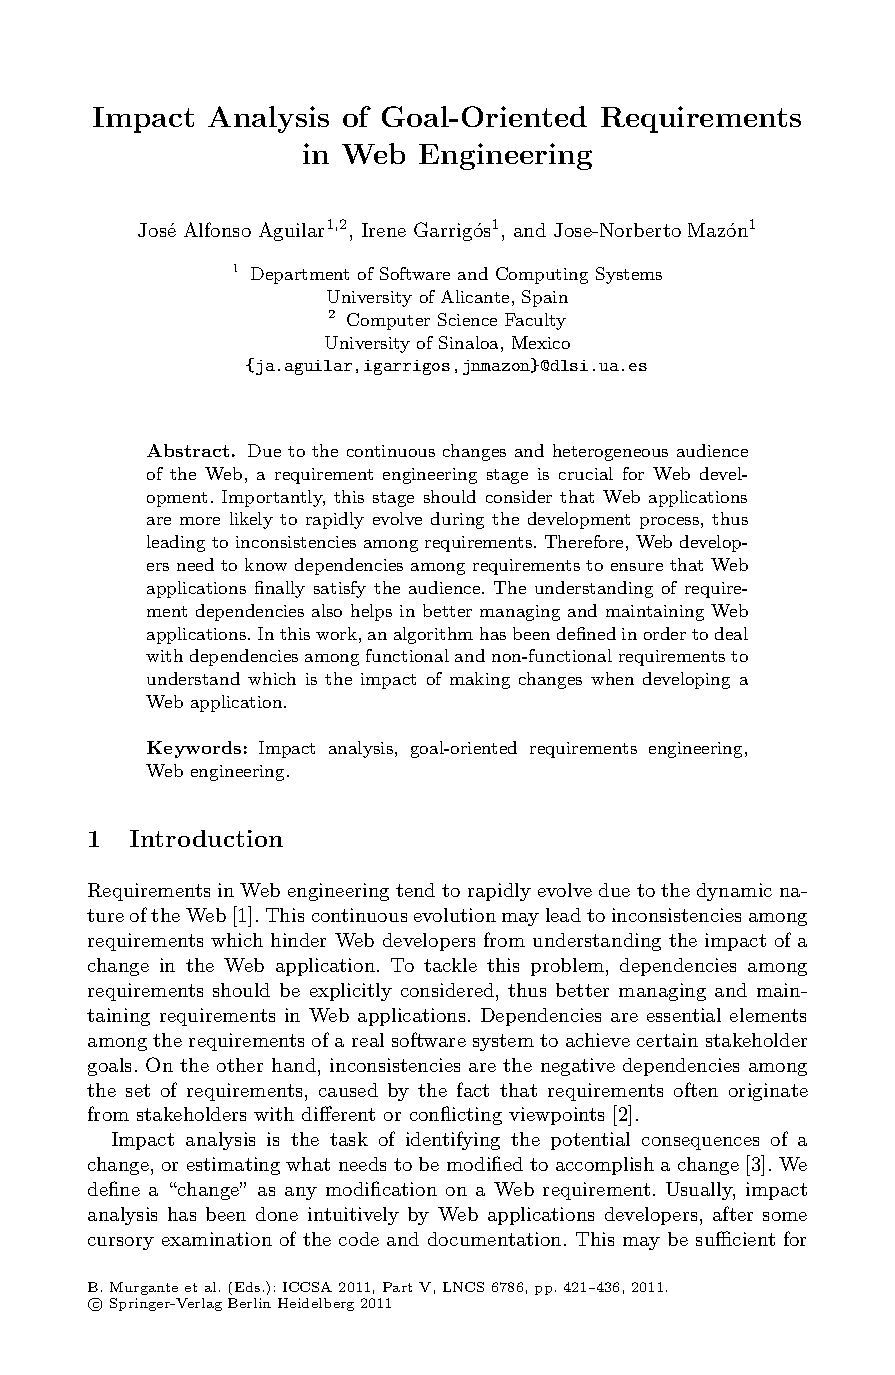
\includepdf[openright=true,pages={1-15}]{papers/ICCSA2011.pdf}
%
